\section{Initial situation} \label{sec:Initial situation}
Formula Student is a worldwide competition where students from different universities are building a formula-style race car, which is either powered by a combustion engine or an electric motor. There are several disciplines for the teams to compete against each other, one of them being \Gls{driverless}. Students must develop an autonomous system for the car to drive fully independent on a given track. For the autonomous system to work appropriately, different components must be implemented. Path planning is one of those components which challenges the software engineers to develop and implement an algorithm that can return to the system a path to drive on. The following chapter introduces the reader to the Formula Student association of the \acrlong{zhaw} (\acrshort{zhaw}) called \acrlong{zur} (\acrshort{zur}). Furthermore, a limited list of related work and implementations is presented.

\subsection{Formula SAE}
In 1980, the idea of an asphalt racing competition was born at the University of Texas by Ron Matthews. Initially called the SAE Mini Indy Competition, it was later renamed to \Gls{formula_sae}. Today, there are many events organized by local associations worldwide. \cite{formula_sae}
These competitions challenge teams of university students to build and participate with formula-style vehicles. They are held worldwide and are one of the biggest student engineering competitions. As of today, there are approximately 600 teams. \cite{sae_student_events}

\textbf{\acrlong{zur}}, formerly known as \acrlong{fszhaw} (\acrshort{fszhaw}), was launched back in 2019, with the first fully functional car finished in 2021. The team is building a new car for the 2022 season, with more than 60 students involved. The new car has seen several improvements in aerodynamics, design, and, most significantly, driverless capabilities. \cite{fszhaw_launch}
Therefore, for the first time in the association's history, the team will compete in the \acrlong{dc} (\acrshort{dc}) category. Both car's are shown in figure \ref{fig:ZUR Racecars}.
The ability to localize itself on an unknown track and optimize a fully known track are critical components of a driverless race car. Therefore, it is essential to research, implement and test various path planning algorithms. A new path planning module must be implemented as part of the newly revised autonomous system, which also includes prediction, localization, and control. The reworked autonomous system will be explained in detail in section \ref{sec:Zurich UAS Racing Autonomous System}.
The team will be competing at Formula Student events in Switzerland, organized by FS Switzerland \cite{fsswitzerland}, Germany, organized by Formula Student Germany \cite{fs_germany}, and Croatia, organized by FS Alpe Adria \cite{fs_alpe_adria}.
\begin{figure}[H]
    \centering
    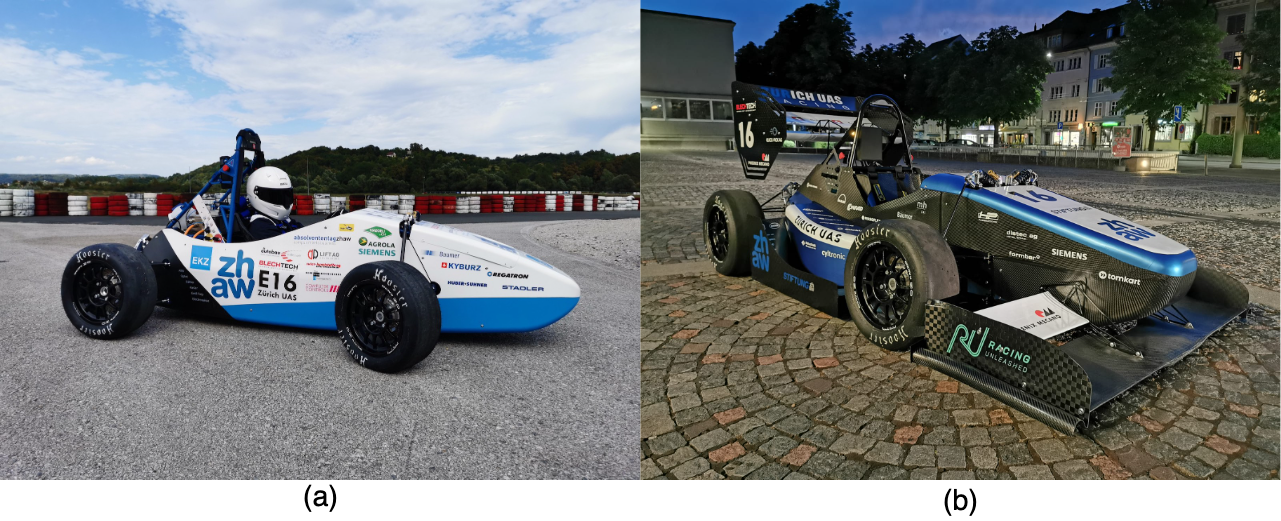
\includegraphics[width=\columnwidth]{ZUR_Racecars.png}
    \caption{Figure (a) shows the first race car developed by \acrshort{zur}, and figure (b) shows the new second race car developed by \acrshort{zur}.}
    \label{fig:ZUR Racecars}
\end{figure}

\subsection{Related Work} \label{sec:Related Work}
PythonRobotics is a Python library hub for a wide range of different implementations in robotics. It varies between arm, aerial, car robotics, and more.
For these robotics segments, it provides an overview of different algorithm implementations, including several path planning algorithms. \cite{python_robotics}
The path planning algorithms differ from different approaches and will be later defined in section \ref{sec:Path Planning Algorithms}.

The first implementation of a path planning algorithm in the team of \acrshort{zur} consisted of middle line detection, path smoothening, and a velocity and acceleration profile. Delaunay-Triangulation was used to evaluate the middle line of the track. E.g., when a cone was not detected, an error rate was considered. The implementation did not cover an algorithm that draws the optimum line considering curves and speed. Furthermore, the overall software architecture must be simpler and easier to understand so that future team members can improve on the work done before. \cite{autopilot_for_formula_student_jerome}

The \acrlong{amz} (\acrshort{amz}), founded by students of the \acrlong{eth} (\acrshort{eth}), \cite{amz_racing_about} have publicly published path planning algorithms and other resources. Algorithms like the \acrshort{rrt} algorithm for track exploration and a \acrlong{mpcc} (\acrshort{mpcc}) for autonomous racing have been implemented. Furthermore, they provide a skeleton for building and implementing driverless algorithms for easier software distribution. \cite{amz_racing_github}

The \acrlong{eufs} (\acrshort{eufs}) team developed an autonomous race car's path planning and control algorithm by a see-think-act cycle method. "See" means what kind of information the sensors and cameras provide. With "think", the processing of the images, sensor data, mapping, localization, and path planning is meant. Furthermore, "act" describes the vehicle's mechanism to steer, accelerate, and brake. \cite{path_planning_and_control_georgiev}
In their report, they specifically mention two algorithms used for path planning: The \Gls{a_star_search_algorithm} and the \Gls{rapidly-exploring_random_tree} (\acrshort{rrt}) algorithm. In the \Gls{darpa_grand_challenge}, all vehicles used various A* Graph Search Algorithms considering the kinematics. Furthermore, the incremental search algorithm \acrshort{rrt} was also used in the path regarding autonomous driving. \cite{darpa_grand_challenge}
Another algorithm is used to control the vehicle, the so-called \acrlong{mppi} (\acrshort{mppi}) algorithm. \cite{model_predictive_path_integration}

\acrlong{eufs} also developed a simulation tool based on \Gls{gazebo}, which is the simulation toolbox for \acrshort{ros} and maintained by the same organization, Open Robotics. \cite{gazebo_simulator} With the help of this application, a simulation of the race with real-world conditions is possible to a certain degree. The simulation was made to test the implementation of various path planning algorithms and other functionalities regarding a driverless system. One of the program's main features helps generate a racetrack based on an image. \acrshort{eufs} also made pre-made CSV files available containing track information for the acceleration and skidpad track used in the Formula Student competitions. Various maps of track drive tracks are also provided. \cite{eufs_path_planning_and_control} \cite{eufs_sim_gitlab}

The \acrlong{tum} (\acrshort{tum}) houses a department named \acrlong{ftm} (\acrshort{ftm}), which developed an optimization algorithm for calculating the most optimal race trajectory of a given route. The algorithm takes a reference line (e.g., the middle line) and the distances to the track's borders as inputs and generates an optimal racing line for the given track. Additionally, an acceleration profile and curvature profile are generated. \cite{minimum_curvature_trajectory_planning} \cite{minimum_time_trajectory_planning} \cite{tumftm_optimization_algoritm} \cite{tumftm_trajectory_planning_helpers}

\acrlong{fsds} (\acrshort{fsds}) is a community project where multiple students from different Formula Student teams have worked on a simulation tool to test driverless system components. The simulation tool is based on Unreal Engine 4 \cite{unreal_engine} and has a \acrshort{ros} bridge to connect algorithm implementations to the simulation tool. It comes with pre-implemented tracks like Acceleration and Skidpad. Additionally, other tracks, which are based on past competitions, are provided. These other tracks help the teams to test the algorithms with real-world-like tracks. \cite{fsds_github}

\section{Problem Definition / Objective / \newline Requirements} \label{sec:Problem Definition / Objective / Requirements}
\subsection{Problem Definition} \label{sec:Problem Definition}
\acrlong{zur}, the university's racing team, has begun its work on its second-generation race car since Fall 2021. With path planning being an integral part of an autonomous car, researching and implementing a new path planning module as part of their new autonomous system is very important. For further information, see the official problem definition in the appendix \ref{problem_definition}.

\subsection{Objective} \label{sec:Objective}
While a path planner has previously been implemented in the team, the functionality and stability of the program are relatively modest. Only an algorithm for exploring an unknown track is given; the optimization of a fully known track is not supported. Additionally, the application has been implemented with a model car in mind and not with the actual race car. With those limitations in mind, it was decided that an entirely new system would be needed. The program was also implemented using ROS 1 and C++, while the new autonomous system will be using ROS 2 with primarily Python. Thus, this thesis aims to research and implement several path planning algorithms that can be adapted to different tracks and driving scenarios, with the end goal of being able to compete in the \acrlong{dc} at various Formula Student events between July and August.

\subsection{Overview} \label{sec:Overview}
The following chapter (\ref{ch:Background}) will convey the required background knowledge on several topics. Topics include Formula SAE and its competitions (\ref{sec:Formula SAE Competitions}), the autonomous system of \acrlong{zur} (\ref{sec:Zurich UAS Racing Autonomous System}), the \acrlong{ros} (\ref{sec:Robot Operating System (ROS)}), the concept of driverless (\ref{sec:Driverless}), and path planning algorithms in general (\ref{sec:Path Planning Algorithms}). During the Approach and Methods chapter (\ref{ch:Approach / Methods}), the design, implementation, verification, and project approach while constructing the path planning system will be elaborated more precisely. A summary of the results will be given in the Results chapter (\ref{ch:Results}), followed by the Discussion and Conclusion chapter (\ref{ch:Discussion Conclusion}), which will review the achieved results from the chapter before.
